\documentclass[]{article}

%opening
\title{Project 3 Numerical Methods}
\author{Dustin O'Brien}

\usepackage{graphicx}
\usepackage{listings}
\usepackage{xcolor}

\lstdefinestyle{mypython}{
	language=Python,
	backgroundcolor=\color{lightgray}, % Background color for the code
	commentstyle=\color{green},        % Style for comments
	keywordstyle=\color{blue},         % Style for keywords
	stringstyle=\color{red},           % Style for strings
	basicstyle=\ttfamily,              % Basic code font style
	showstringspaces=false,            % Don't show spaces in strings
	tabsize=4,                         % Tab size
	breaklines=true,                   % Line breaking
	frame=single                       % Frame the code
}


\begin{document}
	
	\maketitle
	
	\section*{Problem 3c}
	
		
		\section*{Python Code}
		
		
		
		\begin{lstlisting}[style=mypython]
			#Allows usage of math functions
			import math
			#Allows User to type in as Fraction
			from fractions import Fraction
			
			#Function f(x)
			def f(x):
			return math.sin(math.pi * x)
			
			#Takes in user input uses Fraction to convert fraction into something usable than converts that into a decimal
			x = float(Fraction(input("Please Input Your x\n")))
			h = float(Fraction(input("Please Input Your h\n")))
			
			#Formulas for calculating these things Based on Forward Difference
			approx1 = (f(x + h) - f(x)) / h
			error1 = (math.pi ** 2 * h) / 2
			
			#Formulas for calculating Based on Central Difference
			approx2 = (f(x + h) - f(x - h)) / (2 * h)
			error2 = (math.pi ** 3 * h ** 2) / 6
			
			#Outputs
			print("Forward Difference Approximation: ", approx1, " Error: ", error1)
			print("Central Difference Approximation : ", approx2, " Error: ", error2)
			
			
			
		\end{lstlisting}
		
	
	
	\section*{Problem 6a}
	Consider the following equation where $A,B,C$ are all constants
	
	\[Af(x) + Bf(x+h) + Cf(x+2h) = f'(x)\]
	
	Using Taylors Theroem we know
	
	
	\[f(x+h) = f(x) + hf'(x) + \frac{h^2f''(\xi_1)}{2}\]
	\[f(x+2h) = f(x) + 2hf'(x) + 2h^2f''(\xi_2)\]
	Thus,
	\[Af(x) + Bf(x+h) + Cf(x+2h) = Af(x) + Bf(x) + Bhf'(x) + \frac{Bh^2f''(\xi_1)}{2} + Cf(x) + 2Chf'(x) + 2Ch^2f''(\xi_2)\]
	
	\[Af(x) + Bf(x+h) + Cf(x+2h) = Af(x) + Bf(x)+ Cf(x)  + Bhf'(x) + 2Chf'(x) + 2Ch^2f''(\xi_2) + \frac{Bh^2f''(\xi_1)}{2}\]
	
	\[Af(x) + Bf(x+h) + Cf(x+2h) = Af(x) + Bf(x)+ Cf(x)  + Bhf'(x) + 2Chf'(x) + O(h^2)\]
	
	Since, there is no f(x) in final product and 1 f'(x) we know
	
	\[A + B + C = 0\]
	\[Bh + 2Ch = 1\]
	
	
	\[B  = \frac{1-2Ch}{h}\]
	\[A + \frac{1-2Ch}{h} + C = 0\]
	\[A + \frac{1-2Ch+ Ch}{h} = 0\]
	\[A + \frac{1-Ch}{h} = 0\]
	\[A  = -\frac{1-Ch}{h}\]
	\[A  = \frac{Ch-1}{h}\]
	
	Let $C = 1$
	
	\[A  = \frac{h-1}{h}\]
	\[B  = \frac{1-2h}{h}\]
	\[C = 1\]
	
	\section*{Problem 8}
	Consider the function
	
	\[8f(x+h) - 8f(x-h) - f(x+2h) + f(x-2h)\]
	
	Using Taylors Theroem we know,
	
	\[f(x+h)=f(x)+hf'(x)+h^2f''(x)\frac{1}{2} + h^3 f'''(x)\frac{1}{6} + h^4f^{(4)}(x)\frac{1}{24} + h^5f^{(5)}(\xi_1)\frac{1}{120}\]
	
	\[f(x-h)=f(x)-hf'(x)+h^2f''(x)\frac{1}{2} - h^3 f'''(x)\frac{1}{6} + h^4f^{(4)}(x)\frac{1}{24} - h^5f^{(5)}(\xi_2)\frac{1}{120}\]
	
	\[f(x+2h)=f(x)+2hf'(x)+4h^2f''(x)\frac{1}{2} + 8h^3 f'''(x)\frac{1}{6} + 16h^4f^{(4)}(x)\frac{1}{24}+ h^5f^{(5)}(\xi_3)\frac{1}{120}\]
	
	\[f(x-2h)=f(x)-2hf'(x)+4h^2f''(x)\frac{1}{2} - 8h^3 f'''(x)\frac{1}{6} + 16h^4f^{(4)}(x)\frac{1}{24} - h^5f^{(5)}(\xi_4)\frac{1}{120}\]
	
	Inserting these into the original function we get and simplifying all $h^5$ terms which are only multiplied by constants to $O(h^5)$ we get
	
	\[8f(x+h) - 8f(x-h) - f(x+2h) + f(x-2h) = 12hf'(x)+O(h^5)\]
	
	\[\frac{8f(x+h) - 8f(x-h) - f(x+2h) + f(x-2h)+O(h^5)}{12h} = f'(x)\]
	
	\[\frac{8f(x+h) - 8f(x-h) - f(x+2h) + f(x-2h)}{12h}+O(h^4) = f'(x)\]
	
	\section*{Problem 11}
	
	Looking at graph at bottom of page  we notice the staticy error begins to occur around 600 however its worth mentioning that Python doesn't use floating point artihmetic and instead uses arbitrary-precision arthemtic therefor this is a different but likely similar sort of error being caused
	
	\begin{figure}[h]  % "h" means to place the figure "here" in the text
		\centering
		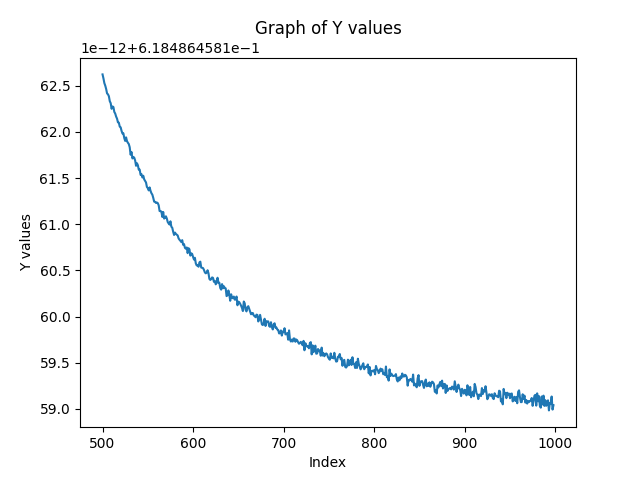
\includegraphics[width=1.5\textwidth]{Figure_1.png}  % Path to the image file
		\caption{Approximation of derivative arctan.}
		\label{fig:example_image}
	\end{figure}
	
	\section*{Problem 12}
	Consider the function
	\[-2f(x)+f(x+h)+f(x-h)\]
	Using Taylor Series we know
	\[f(x+h) = f(x) + h f'(x)\frac{1}{2} +h^2f''(x) +h^3f'''(x)\frac{1}{6} + h^4 f^{(4)}(\xi_1)\frac{1}{24}\]
	
	\[f(x-h) = f(x) - h f'(x)\frac{1}{2} +h^2f''(x) -h^3f'''(x)\frac{1}{6} + h^4 f^{(4)}(\xi_1)\frac{1}{24}\]
	
	Thus,
	
	\[h^2f''(x)\frac{1}{2} + h^4f^{(4)}(\xi_1)\frac{1}{24}+ h^4f^{(4)}(\xi_2)\frac{1}{24}\]
	
	\[h^2f''(x)\frac{1}{2} + h^4(f^{(4)}(\xi_1)\frac{1}{24}+ f^{(4)}(\xi_2)\frac{1}{24})\]
	
	\[h^2f''(x)\frac{1}{2} + O(h^4) = -2f(x)+f(x+h)+f(x-h)\]
	
	\[f''(x) = \frac{-4f(x)+2f(x+h)+2f(x-h) + O(h^4)}{h^2}\]
	
	Therefore,
	\[f''(x) = \frac{-4f(x)+2f(x+h)+2f(x-h)}{h^2} + O(h^2)\]
	
\end{document}